% TeX'ing this file requires that you have AMS-LaTeX 2.0 installed
% as well as the rest of the prerequisites for REVTeX 4.1
%
% It also requires running BibTeX. The commands are as follows:
%
%  1)  latex apssamp.tex
%  2)  bibtex apssamp
%  3)  latex apssamp.tex
%  4)  latex apssamp.tex
%
\documentclass[%
 reprint,
 amsmath,amssymb,
 aps,
]{revtex4-1}

\usepackage{graphicx}% Include figure files
\usepackage{dcolumn}% Align table columns on decimal point
\usepackage[english,ngerman]{babel}
\usepackage{bm}% bold math
%\usepackage[mathlines]{lineno}% Enable numbering of text and display math
%\linenumbers\relax % Commence numbering lines

%\usepackage[showframe,%Uncomment any one of the following lines to test 
%%scale=0.7, marginratio={1:1, 2:3}, ignoreall,% default settings
%%text={7in,10in},centering,
%%margin=1.5in,
%%total={6.5in,8.75in}, top=1.2in, left=0.9in, includefoot,
%%height=10in,a5paper,hmargin={3cm,0.8in},
%]{geometry}

\begin{document}

%\preprint{APS/123-QED}

\title{Data Quality in a Big Data Context}% Force line breaks with O MEASURING DATA Q... ? \\

\begin{abstract}
This article proposes a methodology to model and measure Data Quality in a Big Data context, in particular, a stream of Twitter feeds. We aim to quantify its quality by using a formal system defined in this paper, and use it to classify the users based on the quality of their feeds given a particular hashtag.
\begin{description}
\item[Key words]
Data Quality, Big Data, Information Quality
\end{description}
\end{abstract}

\maketitle

%\tableofcontents

\section{\label{sec:level1}Introduction}

TODO: NEED TO ADD THE PROGRAM ARCHITECTURE AND DECISONS OF WHY IT HAS ITS TOPOLOGY AND TECHNOLOGIES. 


Data Quality is an important topic when dealing with a significant amount of data. This information might come from different sources, in different formats and types and is not guaranteed that any piece of information will equally fit our needs. Poor Data Quality has serious problems when talking about businesses' process, the report of the Data Warehousing Institute (Data Warehousing Institute. Data Quality and the Bottom Line: Achieving Business Success through a Commitment to High Quality Data. http://www.dw-institute.com/) estimates Data quality issues costs U.S. businesses more than 600 billion dollars a year (Data Quality: Concepts, Methodologies and Techniques. Carlo Batini, Monica Scannapieca).

In this paper, we will tackle the Data Quality issue in a Big Data context. To get a vague idea on what Big Data is, think of how many requests are sent by a single cellphone when notifying its location to the Google Maps GPS systems. Now multiply that number by all the users in your area and we have a big amount of data to handle, process and analyze. Multiply it for the number of users in your country, or by all the users in the world. That's a vague idea of what Big Data means.

We will first define what do we mean by \emph{Data Quality}, before going through some general quality dimensions, such as accuracy, completeness, currency, timeliness, volatility, consistency, among others. Then, specify what those dimensions mean in a Big Data context, this is, define models and metrics to measure the  Data Quality dimensions so we can compare a sample from the information stream with others and decide which piece of information best fits our purposes. In order to do this, we will follow the work from \emph{On the Meaningfulness of “Big Data Quality”} by Donatella Firmani, Massimo Mecella, Monica Scannapieco and Carlo Batini. (REF)

Our goal is to define a deterministic methodology to measure Data Quality for each sample of the information stream, so we will formalize the models and metrics defined before in a formal system, with a similar way as DataLog does (ref to DataLog).

With all this information in place, we will conclude with the implementation of this new methodology and the test of two real life examples of Big Data problems in the industry. Finally, we will be able to take a sample from any information stream and decide if the new piece of data will fit our needs better than other.

This article is structured as follows:
\begin{itemize}
  \item \textbf{Data Quality:} What do we mean by \emph{Data quality}? Dimensions and metrics. Structured data vs. unstructured data.
  \item \textbf{Big data:} What do we mean by \emph{Big Data}? Different sources of information. 4Vs.
  \item \textbf{Data Quality in a Big Data context:} Specify dimensions and metrics when dealing with information in a Big Data context.
  \item \textbf{Formalizing Big Data Quality:} Brief introduction to formal systems like DataLog. Formalize the dimensions and metrics defined before using a formal system. Define our new methodology to measure Data Quality in a Big Data context with a formal system.
  \item \textbf{Industrial applications:}: Test our new framework in two industrial problems with different sources of information and different types of data. We will be able to define if a piece of data fits our purposes the best or if it doesn't by measuring its quality.
  \item \textbf{Discussion:} Data Quality of structured data vs. unstructured data. Data Quality of different types of sources.
  \item \textbf{Conclusion and future work}
\end{itemize}

\section{\label{sec:level1}Data Quality}

If we google the term \emph{Data quality} we get about 546,000,000 results, but we can briefly refer to the the term as the level of quality of the data. This is not a trivial concept we can define, so we will first introduce other concepts that will help us understanding the meaning of Data Quality to be used in this paper, such as \emph{dimensions} and \emph{metrics}. But first, let's add some context on what's happening in the world regarding Data Quality manners.

As mentioned in the introduction, the report on Data Quality of the Data Warehousing Institute (REF) estimates that Data Quality problems cost U.S. businesses more than 600 billion dollars a year. Some companies in the tech industry are rising their voices on this issue; IBM's acquisition (2005) of Ascential Software, a data integration tools company, highlights the role of Data Quality in one of their reports: it stays Data Quality and security issues as the leading inhibitors to successful data integration projects (REF). SAP has set up a project for testing in the area of Data Quality with important savings in several internal business processes (REF). Informatica, another leading company on data integration, and Oracle are also relying on Data Quality tools in their products (REFS).

And this is not only taking place in private initiatives but also in public ones. In 2001, the US Government signed into law a new Data Quality legislation (REF) which concerns agencies to report periodically the number and nature of Data Quality complaints received, and how those are being handled. On the other hand, the ISO 8000, the new international standard for Data Quality, published in late 2008 their first sections and is still today under development.

\subsection{\label{sec:level1}Dimensions and Metrics}

Many people confuses the concept of Data Quality with Data Quality \emph{dimensions}, such as accuracy, completeness, consistency or currency. For example, a misspelled name in a field of our system would be an accuracy issue. Each dimension captures a specific aspect included under the general umbrella of Data Quality (frase afanada del libro) and helps us to understand the quality of the data we are analyzing. 

Now, we will introduce some of the Data Quality dimensions to be used in this paper:

\begin{itemize}
  \item \textbf{Accuracy:} Is the closeness between a value v and a value v', considered as the correct representation of the real-life phenomenon that v aims to represent. For example, let's take the case of a person that wanted to type the name "Jhon" but typed "Jhn", here we have an accuracy issue.
  \item \textbf{Completeness:} "The extent to which data are of sufficient breadth, depth, and scope for the task at hand" (REF 205 del libro de calidad). When dealing with relational databases, this may be characterized as the presence/absence and meaning of null values (supposing our schema is complete, this is, we aren't missing values in the schema definition but in the DB registry). For example, let's suppose we want to get chronological order of the Matrix movies that we display in Fig. \ref{fig:completeness}. We may see that "The Matrix Revolutions" lacks of a year of release value, so we encounter a completeness issue there. What if we want to see the directors of this movies from the same table? We cannot, cause there is no attribute in the schema of the table to store that information. This last example is a \emph{schema completeness issue}.
  
  \begin{figure}[h]
    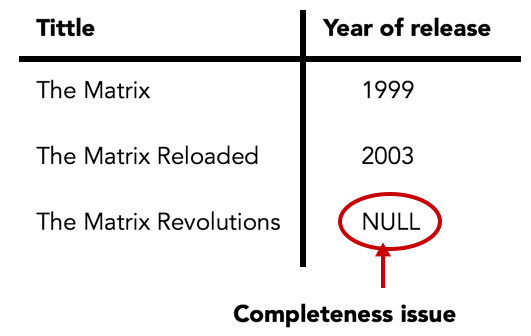
\includegraphics[width=8cm]{movies_table.png}
    \centering
    \caption{Completeness issue example}
    \label{fig:completeness}
  \end{figure}
  
  \item \textbf{Redundancy:} Refers to represent the aspects of reality of matters with the minimal use of informative resources. For example, we have a redundancy in the table of the Figure \ref{fig:redundancy}, where we see the nodes that compose different clusters. There are two methods to calculate the status of the each cluster: by looking at the status of all the nodes in the cluster or by looking at the attribute \emph{status} in the "cluster" table. Redundancy issues might get very complex as we can get the same information from more than one method, and the result of each one may differ, like the case of the cluster 3, which has is status as "RUNNING", but the respective nodes are not "STOPPED".
  
  \begin{figure}[h]
    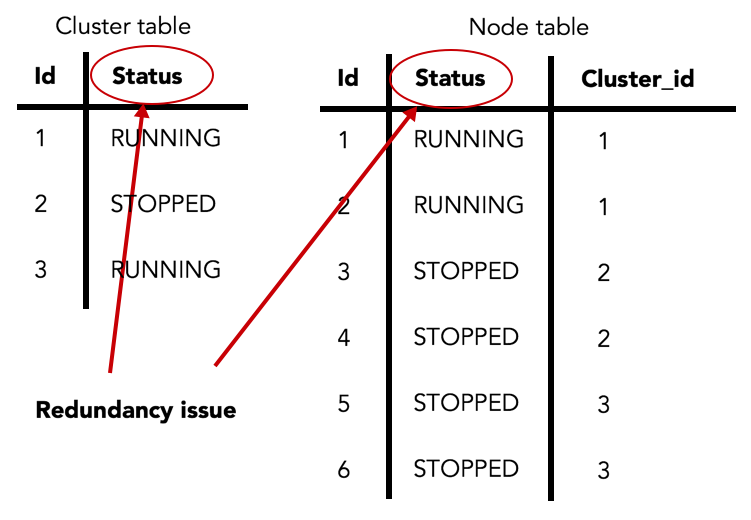
\includegraphics[width=8cm]{redundancy.png}
    \centering
    \caption{Redundancy issue example}
    \label{fig:redundancy}
  \end{figure}
  
    \item \textbf{Consistency:} Refers to the capability of the information to comply without contradictions to all the rules defined in the system where the information relies. For example, in a relational database we set some constraints in the schema to make sure our data is consistent, like Foreign Key constraints between entities. Another example is the mismatch of the status of the cluster in the Figure \ref{fig:redundancy}, where its nodes appear as "STOPPED", but the cluster as "RUNNING". Besides the redundancy issue in that database, there is \emph{consistency} issue.
    
  \item \textbf{Readability:} Refers to the ease of understanding of information. For example, suppose we are scanning a hand written paragraph and some of the characters are not well defined, as seen in Figure \ref{fig:readability}. 
  
  \begin{figure}[h]
    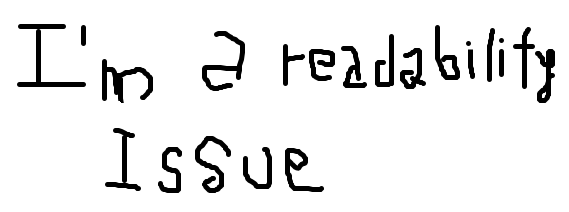
\includegraphics[width=8cm]{readability.png}
    \centering
    \caption{Readability issue example}
    \label{fig:readability}
  \end{figure}
  
  \item \textbf{Accessibility:} Also called availability, is related to the ability of the user to access the information.
  
  \item \textbf{Trust:} Including reliability, focuses on how much  we trust the information source and therefor believe the data is reliable. If we would want to see how good a movie is, we could rely on Facebook or Tweeter posts from regular people, but a different source like www.imdb.com might give us more reliable data. 
  
  \item \textbf{Usefulness:} Is related to the advantage the user gains from the use of information. For example, let's see the scans taken to \emph{The Garden of Earthly Delights} by Hieronymus Bosch we show in Figure \ref{fig:usefulness}: if we'd want to take advantage of the details this painter put on his drawings, we should use the image with the highest contrast vs. the other one.
  
  \begin{figure}[h]
    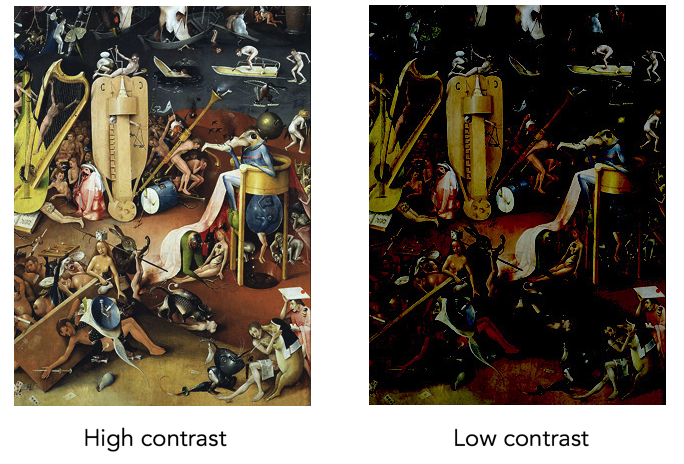
\includegraphics[width=8.8cm]{usefullness.png}
    \centering
    \caption{Usefulness issue example}
    \label{fig:usefulness}
  \end{figure}
\end{itemize}

Now we are familiar with some Data Quality dimensions, but this is not enough. How could we use this clusters of Data Quality in order to see if a piece of data is better than other? We need a way to \emph{quantify} these dimensions, and is for this purpose that we introduce the concept of \emph{metrics} of Data Quality dimensions: \emph{metrics} refer to one or more measurement methods of Data Quality dimensions. We won't dig here on the metrics to be used on this paper but in later sections where we first define which quality dimensions best fit a Big Data problem.

\subsection{\label{sec:level1}Structured vs. Unstructured data}

There is a classification of information that bases on the representation of the data. We may find three types of data that are commonly distinguished here:

\begin{itemize}
  \item \textbf{Structured:} Each piece of information has an associated fixed and formal structure. This is the case of relational databases.
  \item \textbf{Semi structured:} The structure of the data has some degree of flexibility. An example is an XML file that doesn't have an associated XML schema definition, or a JSON response from an API which structure is not 100\% defined.
  \item \textbf{Unstructured:} There is no specific structure or domain types for the data. This is the case of text expressed in natural language.
\end{itemize}

\section{\label{sec:level1}Big Data}

We will say that we are working in a \emph{Big Data} context if the data sets involved in our job are too large to store, analyze, handle or process for the regular tools. For example, suppose all the tweets that are made by all the Tweeter users of the hole world in a day. That's a significant amount of data.

According to the report \emph{Big Data, Bigger Digital Shadows, and Biggest Growth in the Far East}(https://www.emc.com/collateral/analyst-reports/idc-digital-universe-united-states.pdf) by the IDC Go-To-Market Services (February 2013), the size of the data stored in all the US, this is, the digital bits created, replicated and consumed each year in the country, is expected to grow from 898 exabytes to 6.6 zettabytes between 2012 and 2020, or more than 25\% a year, which means it will double about every three years, as seen in Figure \ref{fig:data-increase}.

\begin{figure}[h]
  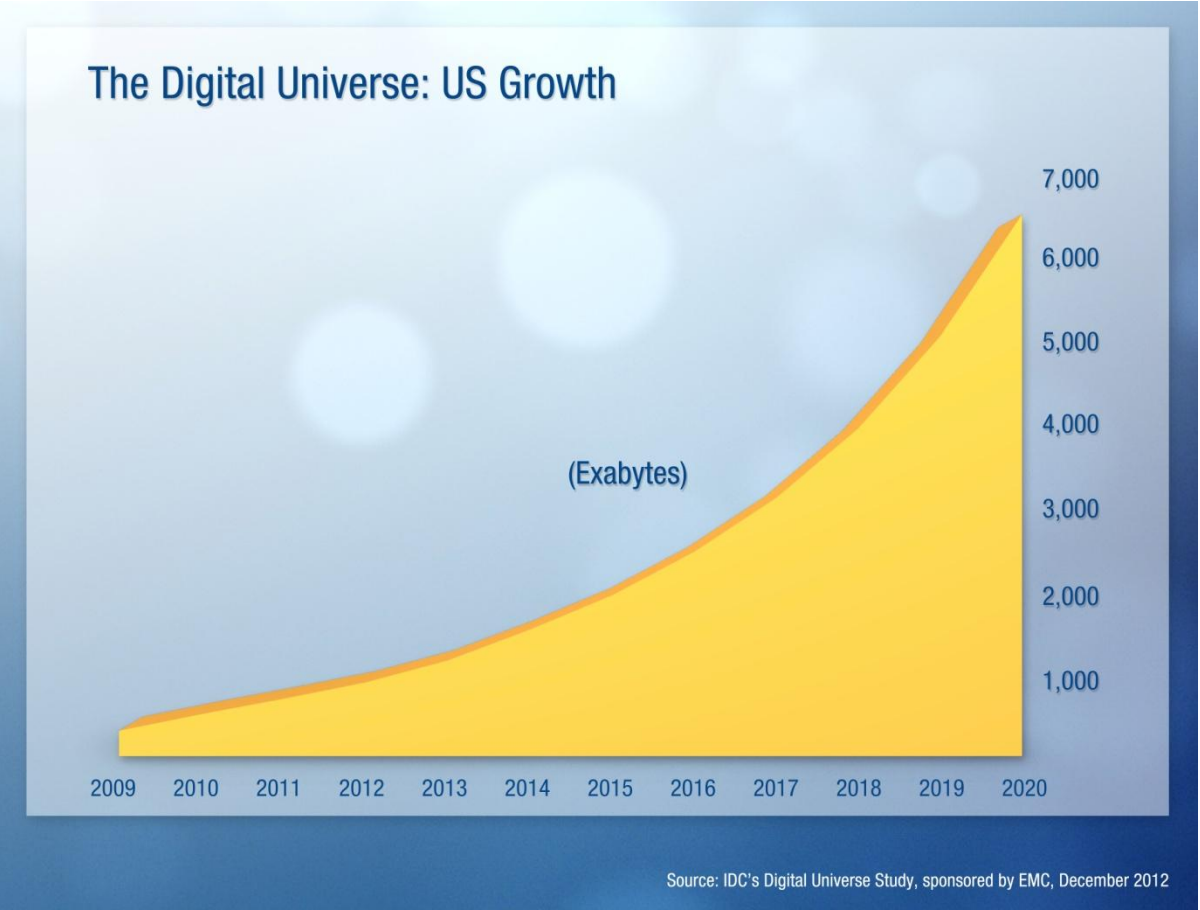
\includegraphics[width=8.8cm]{data-increase.png}
  \centering
  \caption{US data growth during time}
  \label{fig:data-increase}
\end{figure}

\subsection{\label{sec:level1}The 4 Vs}

There are 4 famous features of \emph{Big Data} called "the 4 Vs", as these are 4 characteristics that starts with a "v". These are:

\begin{itemize}
  \item \textbf{Volume:} Refers to size of the generated and stored data.
  \item \textbf{Velocity:} Refers to the data provisioning and processing speed. For example, the record of the amount of Tweets sent per second (TPS) is of 143,199 TPS, on August 2013. (REF a https://blog.twitter.com/2013/new-tweets-per-second-record-and-how)
  \item \textbf{Variety:} Refers to the heterogeneity of the data representation, provisioning method and semantic interpretation. The type and nature of the data.
  \item \textbf{Veracity:} The reliability of the data might differ a lot in the same information stream. This is reflected in inconsistencies and quality issues within the data.
\end{itemize}

Some authors might add more Vs to these list, like variability, but we will keep with these 4.

\subsection{\label{sec:level1}The types of sources of the data}

According to the UNECE (United Nations Economic Commission for Europe)(REF a http://www1.unece.org/stat/platform/display/bigdata/Classification+of+Types+of+Big+Data), there are three main categories of the source of the data when talking about Big Data: human sourced (i.e., tweets or Facebook posts), process mediated (i.e., banking records) and machine generated (i.e., an earthquake monitor). This classification is very important, as there will be different treatments to measure Data Quality
depending on the source type. But before, let's describe each in particular:

\begin{itemize}
  \item \textbf{Social Networks (human-sourced information):} This is the information people provides via text, photographs or videos. Usually, this information lacks of a fixed structure, like the texts written in natural language. Therefor, we may say that the information streamed here is loosely structured and often ungoverned. Examples are social networks posts (Facebook, Twitter), YouTube videos or e-mails.
  \item \textbf{}
\end{itemize}

\section{\label{sec:level1}Data Quality in Big Data}

Specify dimensions and metrics in a Big Data context from the paper.
Summarize a system to measure data quality for ANY piece of data in a big data context.

\section{\label{sec:level1}A formal system to measure Data Quality}

Some words about datalog and defining axioms and rules in that way.
Define data quality in a formal system.
Define logical rules to measure data quality in a big data context based on what we saw.

Processed mediated sources examples:
Big data Processed mediated sources: https://data.gov.uk/ CVS with the hole DB of payments in lots of shops.

From APIs (): movies rates from http://api.rottentomatoes.com/ or imdb api.

Human sources information:
Stream of tweets API

Monitors:
http://earthquake.usgs.gov/fdsnws/event/1/

See if the people liked or not some movies based on the rottentomates api and imdb api (and we can include tweets of people).
See earthquake monitors data and tweets that may talk about an earthquake in that area.

\end{document}
%
% ****** End of file apssamp.tex ******